\documentclass[
    11pt,
    a4paper,
    sfdefaults=false,
    toc=chapterentrywithdots,
    oneside,  % Ensures consistent margins
    openany,  % No blank pages between sections
    titlepage,
    parskip=half,
    headings=normal,  % reduces heading size
    listof=totoc,
    bibliography=totoc,
    index=totoc,
    captions=tableheading,  % caption below table
    listof=flat,
    final
]{scrbook}


% details about your thesis
\newcommand{\titel}{CYBRAIL}
\newcommand{\artderarbeit}{IT-Projekt}  % {Bachelorarbeit,Masterarbeit}
\newcommand{\autor}{Mattis Krämer, Robin Rosner, Pascal Blank}
\newcommand{\studiengang}{Bachelor Informatik}  % {Informatik,Wirtschaftsinformatik,Medieninformatik}
\newcommand{\matrikelnr}{,,3646070}
\newcommand{\erstgutachter}{Dr. Martin Geier}
%\newcommand{\zweitgutachter}{Prof.\,Dr.~Donald Duck}
%\newcommand{\betreuer}{M.Sc.\,~Martina Schmidt}
%\newcommand{\unternehmen}{Musterfirma GmbH}
\newcommand{\logo}{figures/TH-Nuernberg-RGB.png}
\newcommand{\keywords}{hot, fuzz}
\newcommand{\creationsemester}{SS2024 - WS2425}
\newcommand{\submissiondate}{06.01.2025}

% custom head and foot
\usepackage[automark]{scrlayer-scrpage}
\pagestyle{scrheadings}
\ihead{\headmark}
\chead{}
\ohead{\pagemark}
\renewcommand*\chaptermarkformat{\chapappifchapterprefix{\ }% 
  \thechapter.\enskip}

\RedeclareSectionCommand[tocindent=0pt]{section}
\RedeclareSectionCommand[tocindent=0pt]{subsection}
%\RedeclareSectionCommand[tocnumwidth=70pt]{chapter}

\usepackage{scrhack}

% other packages
\usepackage[utf8]{inputenc}
\usepackage{float}
\usepackage{tabularx}
\usepackage{pdflscape}
\usepackage[T1]{fontenc}
\usepackage{lmodern,relsize,textcomp,csquotes}
\usepackage{amsmath,amsfonts}
\usepackage[english, ngerman]{babel}  % flip for German thesis
\usepackage[final]{graphicx}
\usepackage{setspace,geometry,xcolor}
\usepackage{makeidx}
\usepackage{paralist,ifthen,todonotes}
\usepackage{url}
\usepackage[toc]{glossaries}
\usepackage{pdfpages}

% table setup
\usepackage{longtable}
\usepackage{array}
\usepackage{ragged2e}
\usepackage{lscape}


% pdf hyperref

\usepackage[
    bookmarks=true,
    bookmarksopen=true,
    bookmarksnumbered=true,
    bookmarksopenlevel=1,
    pdftitle={\titel},
    pdfauthor={\autor},
    pdfcreator={\autor},
    pdfsubject={\titel},
    pdfpagelabels=true,
    colorlinks=true,       % Links are colored
    linkcolor=blue,        % Internal link color
    urlcolor=blue,         % External link color
    citecolor=blue,        % Citation link color
    filecolor=blue,        % File link color
    menucolor=blue,        % Menu link color
    plainpages=false,
    hypertexnames=true,
    linktocpage=true,
]{hyperref}

\usepackage[
    backend=biber,
    style=alphabetic,
    maxbibnames=10,
]{biblatex}

% configure your listings style
\usepackage{listings}
\lstset{
	tabsize=3,
	extendedchars=true,
	frame=single,
	showstringspaces=true,
	numbers=left,
	numberstyle=\small,
	breakautoindent=true
}

\addbibresource{refs.bib}

% page setup
% \setlength{\topskip}{\ht\strutbox}
% Adjust the geometry and page layout
\geometry{paper=a4paper,left=2.5cm,right=2.5cm,top=3.0cm,bottom=3.0cm,bindingoffset=0cm}
\setstretch{1.5}
\frenchspacing
\clubpenalty = 10000
\widowpenalty = 10000 
\displaywidowpenalty = 10000

% some commands
\newcommand{\ua}{\mbox{u.\,a.\ }}
\newcommand{\zB}{\mbox{z.\,B.\ }}
\newcommand{\dahe}{\mbox{d.\,h.,\ }}
\newcommand{\bzw}{\mbox{bzw.\ }}
\newcommand{\bzgl}{\mbox{bzgl.\ }}
\newcommand{\eg}{\mbox{e.\,g.\ }}
\newcommand{\ie}{\mbox{i.\,e.\ }}
\newcommand{\wrt}{\mbox{w.\,r.\,t.\ }}
\newcommand{\etal}{\mbox{\emph{et\,al.\ }}}


% TODO remove if not needed...
%\usepackage{blindtext}

% load glossary entries
\makenoidxglossaries
\loadglsentries{glossary}

\begin{document}


\setcounter{secnumdepth}{3}  % numerate subsections
\setcounter{tocdepth}{2}  % ...but don't include them in toc

\frontmatter
\include{cover}

% download the following form (requires VPN) and complete it (hit save in your editor)
% https://intern.ohmportal.de/fileadmin/Public_Docs/SB/SB_0009_FO_Pruefungsrechtliche_Erklaerung_und_Erklaerung_zur_Veroeffentlichung_der_Abschlussarbeit_public.pdf
%\includepdf{SB_0009_FO_Pruefungsrechtliche_Erklaerung_und_Erklaerung_zur_Veroeffentlichung_der_Abschlussarbeit_public.pdf}\cleardoublepage


%\chapter{Einleitung} \label{ch:einleitung}

Im Rahmen dieses IT-Projekts wurde das System CYBRAIL entwickelt, um die Integrität und Transparenz akademischer Prüfungen signifikant zu verbessern. Mit der fortschreitenden Digitalisierung von Prüfungsprozessen gewinnt der Einsatz von Tools wie dem Safe Exam Browser (SEB) zunehmend an Bedeutung, da sie gewährleisten, dass Prüfungen unter fairen Bedingungen durchgeführt werden und unerlaubte Hilfsmittel ausgeschlossen bleiben. Allerdings stellt die Auswertung der durch den SEB generierten Protokolle (Logs) bislang eine erhebliche Herausforderung dar, insbesondere wenn es darum geht, potenziell verdächtige Aktivitäten in Echtzeit zu identifizieren und adäquat zu reagieren.

Bisher wurde der SEB primär zur Abschreckung von Studierenden verwendet, ohne die generierten Logs systematisch auszuwerten oder zu überprüfen, ob Studierende Wege gefunden haben, die Sicherheitsvorkehrungen des SEB zu umgehen. Diese Lücke birgt das Risiko, dass unrechtmäßige Aktivitäten unentdeckt bleiben und somit die Integrität der Prüfungsergebnisse gefährdet wird.

Das zentrale Ziel von CYBRAIL ist es, diesen Mangel durch die Automatisierung des Prüfungsprozesses zu beheben und den verantwortlichen Professoren eine effiziente, möglichst in Echtzeit ablaufende Kontrolle und Auswertung der SEB-Logs zu ermöglichen. Dies umfasst die Entwicklung von Algorithmen zur automatisierten Analyse und Klassifizierung der Log-Daten, um Verdachtsfälle unerlaubter Mittel schnell und präzise zu erkennen und gleichzeitig entsprechende Beweismittel bereitzustellen. Ein weiteres wichtiges Merkmal von CYBRAIL ist die Bereitstellung einer modularen Systemarchitektur mit flexiblen Schnittstellen, die es ermöglicht, weitere Prüfmechanismen bei Bedarf problemlos zu integrieren.

Durch diese Lösung sollen sowohl die Zuverlässigkeit und Transparenz des Prüfungsprozesses als auch die Nachvollziehbarkeit der Prüfungsergebnisse erheblich gesteigert werden.

\tableofcontents

\mainmatter

\chapter{Einleitung} \label{ch:einleitung}

Im Rahmen dieses IT-Projekts wurde das System CYBRAIL entwickelt, um die Integrität und Transparenz akademischer Prüfungen signifikant zu verbessern. Mit der fortschreitenden Digitalisierung von Prüfungsprozessen gewinnt der Einsatz von Tools wie dem Safe Exam Browser (SEB) zunehmend an Bedeutung, da sie gewährleisten, dass Prüfungen unter fairen Bedingungen durchgeführt werden und unerlaubte Hilfsmittel ausgeschlossen bleiben. Allerdings stellt die Auswertung der durch den SEB generierten Protokolle (Logs) bislang eine erhebliche Herausforderung dar, insbesondere wenn es darum geht, potenziell verdächtige Aktivitäten in Echtzeit zu identifizieren und adäquat zu reagieren.

Bisher wurde der SEB primär zur Abschreckung von Studierenden verwendet, ohne die generierten Logs systematisch auszuwerten oder zu überprüfen, ob Studierende Wege gefunden haben, die Sicherheitsvorkehrungen des SEB zu umgehen. Diese Lücke birgt das Risiko, dass unrechtmäßige Aktivitäten unentdeckt bleiben und somit die Integrität der Prüfungsergebnisse gefährdet wird.

Das zentrale Ziel von CYBRAIL ist es, diesen Mangel durch die Automatisierung des Prüfungsprozesses zu beheben und den verantwortlichen Professoren eine effiziente, möglichst in Echtzeit ablaufende Kontrolle und Auswertung der SEB-Logs zu ermöglichen. Dies umfasst die Entwicklung von Algorithmen zur automatisierten Analyse und Klassifizierung der Log-Daten, um Verdachtsfälle unerlaubter Mittel schnell und präzise zu erkennen und gleichzeitig entsprechende Beweismittel bereitzustellen. Ein weiteres wichtiges Merkmal von CYBRAIL ist die Bereitstellung einer modularen Systemarchitektur mit flexiblen Schnittstellen, die es ermöglicht, weitere Prüfmechanismen bei Bedarf problemlos zu integrieren.

Durch diese Lösung sollen sowohl die Zuverlässigkeit und Transparenz des Prüfungsprozesses als auch die Nachvollziehbarkeit der Prüfungsergebnisse erheblich gesteigert werden.
\chapter{Projektziele} \label{ch:projektziele}
\chapter{Projektverlauf und Meilensteine} \label{ch:projektverlauf}
Dieses Kapitel beschreibt die einzelnen Entwicklungsschritte und die dadurch erreichten Meilensteine unserer Sprints.

\section{Anforderungs- und Risikoanalyse}
Im ersten Sprint haben wir uns mit der Definition der Anforderungen (Requirements) beschäftigt. 
Ziel war es, festzulegen, welche Aspekte unser Projekt abdecken soll und welche Eigenschaften möglicherweise unrealistisch oder optional sind, um einen klaren Fokus zu setzen. 
Eine detailliertere Beschreibung der Anforderungen findet sich in Kapitel \ref{ch:projektziele}.\\
\\
Gleichzeitig mit der Festlegung der Anforderungen haben wir uns ebenfalls mit den daraus resultierenden Risiken auseinandergesetzt. 
Hierbei stand die Frage im Vordergrund, welche Fehlschläge am wahrscheinlichsten und gravierendsten sein könnten. 
Besonders besorgniserregend waren die Risiken in Bezug auf die Beschaffung der Logdateien und den Datenschutz. 
Eine genauere Beschreibung der Risikobewertung findet sich ebenfalls in Kapitel \ref{ch:Risikoanalyse}.

\section{Programmentwurf und Architekturentwurf}
Unser zweiter großer Meilenstein war die Ausarbeitung eines möglichen Programmentwurfs, also der strukturelle Aufbau des Programms.\\
\\
Der Entwurf des Programms sowie die Architektur von \gls{cybrail} basieren auf einer klaren Strukturierung der Funktionalitäten, um eine effiziente und erweiterbare Lösung zu gewährleisten. 
Im folgenden Abschnitt wird der Architekturentwurf näher erläutert, gefolgt von einem detaillierten Blick auf die wichtigsten Klassen und deren Interaktionen.

\subsection{Architekturentwurf}

Das Architekturdiagramm (siehe Abbildung \ref{fig:Architektur}) verdeutlicht die modulare Struktur des Log Processing Systems von CYBRAIL, das in zwei Hauptbereiche unterteilt ist: den \textit{InfoPrep}-Bereich und die \textit{TestingPipeline}.

Im \textbf{InfoPrep}-Bereich werden die eingehenden Logdaten vorverarbeitet. Der wesentliche verbleibende Bestandteil dieses Bereichs ist der \texttt{LogParser}, der die Logs in ein standardisiertes JSON-Format umwandelt, das für die weitere Verarbeitung verwendet wird. Die vorverarbeiteten Daten werden dann an die \textbf{TestingPipeline} weitergeleitet.

Die \textbf{TestingPipeline} führt die eigentlichen Tests auf den vorverarbeiteten Logs durch. Dabei kommen verschiedene Module zum Einsatz, die auf unterschiedliche Anomalien testen. Diese umfassen: \begin{itemize} \item \textbf{MLAnomalyDetector:} Nutzt Machine-Learning-Modelle, wie zum Beispiel zur Erkennung automatischen Tippens (FastTyping Detection). \item \textbf{RuleBasedAnomalyDetector:} Führt regelbasierte Anomalieerkennungen durch, wie die VM-Erkennung (VM Detection) oder die Erkennung mehrerer Bildschirme (Number of Displays Detection). \end{itemize}

Am Ende des Prozesses werden alle Ergebnisse von der \texttt{ResultAggregator}-Komponente gesammelt und zu einem Gesamtbericht zusammengeführt. Dieser Bericht wird anschließend durch die \texttt{Output}-Komponente ausgegeben oder gespeichert.

Durch diese modulare Architektur kann das System flexibel erweitert werden, indem neue Testmodule hinzugefügt oder bestehende angepasst werden. Ebenso bleibt das Parsing der Logs flexibel, um neue Logformate zu unterstützen.

\begin{landscape} 
  \begin{figure}[h] \centering 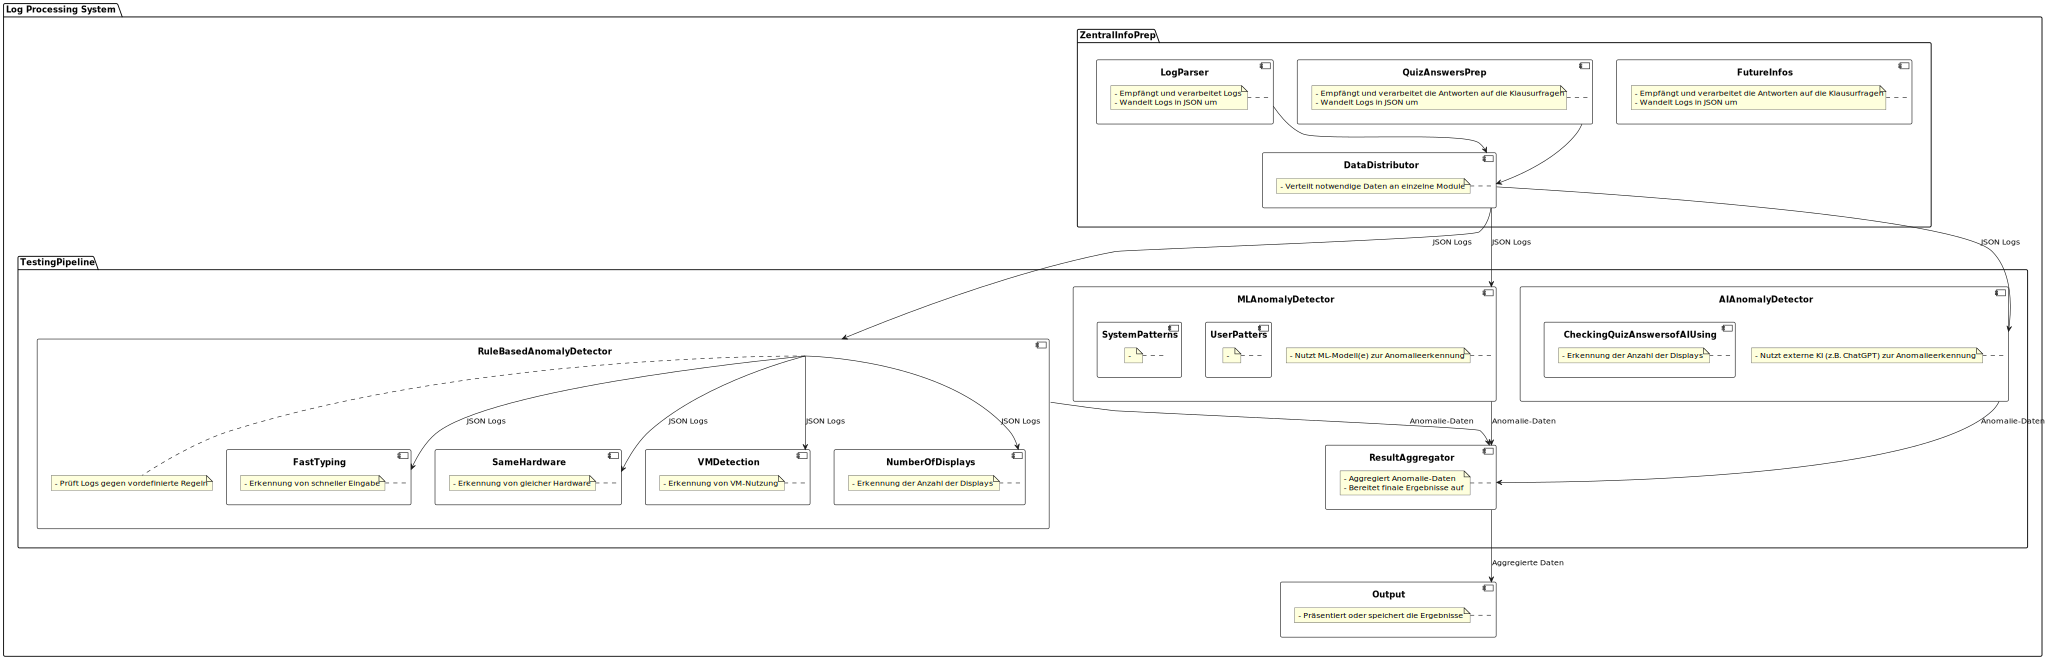
\includegraphics[width=1.5\textwidth]{figures/CybrailArchitektur.pdf} \caption{Architekturdiagramm des Log Processing Systems von CYBRAIL} \label{fig:Architektur} \end{figure} \end{landscape}

\subsection{Programmentwurf}

Das Klassendiagramm (siehe Abbildung \ref{fig:Klassen}) zeigt das Log Processing System von CYBRAIL aus einer objektorientierten Perspektive. Die zentralen Klassen und deren Funktionen sind: \begin{itemize} \item \texttt{LogParser:} Verantwortlich für das Einlesen und Umwandeln von Logdateien in das JSON-Format. \item \texttt{DataDistributor:} Verteilt die vorverarbeiteten Daten an die verschiedenen Testmodule in der TestingPipeline. \item \texttt{RuleBasedAnomalyDetector:} Prüft die Logs auf Basis vordefinierter Regeln, wie der Erkennung von VM-Nutzung oder mehreren Bildschirmen. \item \texttt{MLAnomalyDetector:} Setzt Machine-Learning-Modelle zur Erkennung von Anomalien, wie schnellem Tippen, ein. \item \texttt{ResultAggregator:} Aggregiert die Ergebnisse aller Anomaliedetektoren und erstellt einen finalen Bericht. \item \texttt{Output:} Gibt die gesammelten Ergebnisse aus oder speichert sie. \end{itemize}

Die modulare Struktur des Systems ermöglicht es, die einzelnen Testmodule unabhängig voneinander zu entwickeln und zu erweitern, ohne das Gesamtsystem zu beeinträchtigen. Dies erleichtert auch zukünftige Anpassungen und Erweiterungen.

\begin{landscape} \begin{figure}[h] \centering 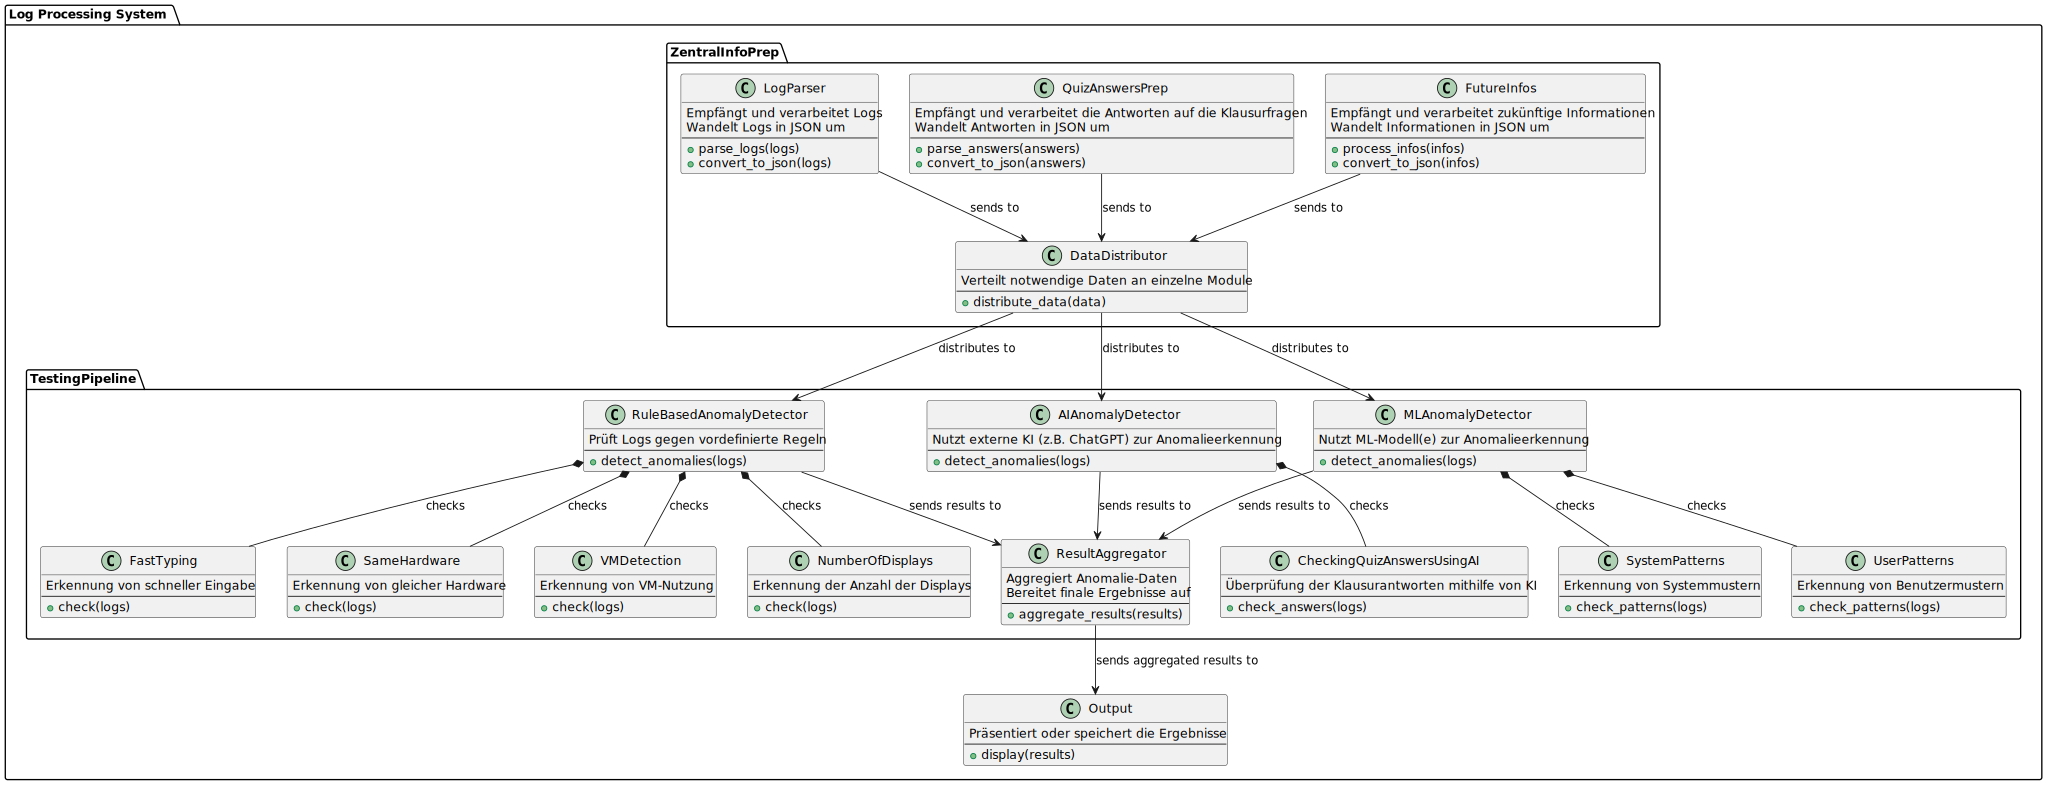
\includegraphics[width=1.5\textwidth]{figures/CybrailClassdiagramm.pdf} \caption{Klassendiagramm des Log Processing Systems von CYBRAIL} \label{fig:Klassen} \end{figure} \end{landscape}

\subsection{Zusammenfassung}

Der Architektur- und Programmentwurf von CYBRAIL zeigt einen modularen Ansatz, der es ermöglicht, das System flexibel zu erweitern und an neue Anforderungen anzupassen. Die klare Trennung von Vorverarbeitung, Anomalieerkennung und Ergebnisaggregation gewährleistet, dass das System sowohl effizient arbeitet als auch gut skalierbar ist. Neue Testmodule und Anpassungen am Logparsing können einfach integriert werden, ohne die bestehende Systemarchitektur zu beeinflussen.

\section{Logparsing und erstes MVP}
Zu Beginn war es wichtig, die eigentlichen Daten, mit denen wir arbeiten wollten, in ein computerlesbares Format zu bringen und somit ein erstes \gls{mvp} zu erstellen.\\
\\
Wir haben einen modularen Ansatz entwickelt, der mithilfe eines Strategy Patterns die unterschiedlichen Arten von Logs – sowohl die der \gls{seb} als auch andere Logtypen – unterscheiden kann und einfach um neue Logtypen erweiterbar ist. 
Dieses Modul nimmt alle Logdateien als Input, identifiziert den Logtyp anhand des Dateinamens und wendet schließlich die passende Strategie an, um das Log in parsierbare \gls{json}-Dateien zu konvertieren, welche später als Grundlage für die Analysen dienen.\\
\\
Für einen ersten Test haben wir außerdem ein Python-Modul entwickelt, das die geparsten Logs von einem Studenten einliest und anhand des Systemnamens erkennt, ob es sich dabei um eine virtuelle Maschine (VM) handelt.\\
\\
Beide Funktionalitäten haben wir in ein erstes \gls{mvp} integriert, das wir in Go geschrieben haben. Dieses \gls{mvp} konnte ein Set von Logdateien parsen, das erste Modul darauf ausführen und einen Status zurückmelden.\\
\\
Für die Kommunikation zwischen dem Hauptprogramm und den Modulen haben wir uns auf die Eingabe von Argumenten und die Ausgabe eines parsierbaren Outputs über \texttt{std::out} geeinigt.

\section{UI und Batchverarbeitung}
Bisher konnte unser Tool nur über die Konsole bedient werden. 
Um die Bedienung zu vereinfachen, haben wir uns entschieden, es mit einer Weboberfläche auszustatten. 
Dies haben wir direkt aus Go heraus umgesetzt, indem wir einige Methoden in API-Calls refaktoriert haben, um Programm-Ein- und Ausgaben zu realisieren.\\
\\
Zeitgleich wurde das Programm erweitert, um Logdateien von beliebig vielen Studierenden auszuwerten und sowohl ein Gesamtergebnis als auch Einzelauswertungen zu erstellen. 
Hierfür wurde eine Programmhilfe entwickelt, die zunächst auf der Konsole den Benutzer unterstützte, alle Logs den richtigen Studierenden mit Namen und Matrikelnummer zuzuordnen. 
Im Verlauf wurde diese Funktionalität auch in die Webversion portiert. Über einen einfachen Knopfdruck konnten alle Logs eingesehen und den Studierenden zugeordnet werden. 
Sobald alle Logs zugeordnet waren, startete das Webinterface eine Analyse für jeden Studierenden und sammelte die Resultate aus allen Modulen, um diese mit detaillierten Auffälligkeiten zu präsentieren.\\
\\
Um Auffälligkeiten über \texttt{std::out} ausführlich zurückzugeben, wurde ein \gls{json}-Schema entwickelt, das genau beschreibt, welche Stelle die Auffälligkeit enthält und was daran auffällig ist.\\
\\
Des Weiteren wurde eine standardisierte Modulkonfiguration eingeführt, mit der Einstellungen für einzelne Module festgelegt werden können, wie zum Beispiel Empfindlichkeit, Keywords etc. Die Anpassung dieser Konfigurationen wurde ebenfalls in das Webinterface integriert. Diese Einstellungen sind generell vorhanden, und das \gls{ui} baut sich automatisch auf Grundlage der Konfigurationen auf, die in der jeweiligen Datei für ein Modul gefunden werden.\\
\\
Neben der Weiterentwicklung von Modulen, um Auffälligkeiten wie Netzwerkänderungen, Bildschirmaktivitäten oder Integritätschecks zu demonstrieren, wurde auch eine Python-Bibliothek entwickelt, um die einzelnen Module zu vereinheitlichen und doppelten Code zu refaktorisieren. 
In jedem Modul sind das Einlesen der Logdateien und der Modulkonfigurationen sowie die Rückgabe von Auffälligkeiten einheitlich gestaltet.

\section{Client-App und KI-Auswertung} 
Eines unserer ersten Ziele war es, sowohl KI-generierte Inhalte als auch automatisches Tippen zu erkennen. 
Die Erkennung von \gls{ki}-generierten Inhalten mussten wir jedoch ausschließen, da wir hierfür die Antworten aller Studierenden zusätzlich aus Moodle hätten extrahieren müssen.\\
\\
Für die Erkennung, ob automatisches Tippen verwendet wurde – eine Alternative zu Copy-Paste – haben wir zwei Szenarien identifiziert:
\begin{enumerate} 
\item Anschläge mit konstanten Zeitabständen 
\item Anschläge mit variierenden Zeitabständen, die unauffälliger wirken 
\end{enumerate}
Um beide Fälle erkennen zu können, haben wir uns dazu entschieden, eine \gls{ki} zu trainieren, die mit hoher Wahrscheinlichkeit diese beiden Szenarien als potenzielle Betrugsversuche erkennt. 
Dazu wurde ein Programm geschrieben, das automatisch getippte Daten generiert. 
Als Input dienten \gls{ki}-generierte Texte, die in Wortwahl, Grammatik etc. den Klausurantworten ähneln sollten. 
Diese Texte wurden aufgeteilt: Ein Teil wurde mit konstanten Intervallen aufgezeichnet, der andere Teil mit Variationen, die durchschnittliches menschliches Tippverhalten nachahmen sollten.\\
\\
Als Grundlage für die Verarbeitung haben wir ein Format entwickelt, das lediglich die Zeit zwischen jedem Tastenanschlag speichert. 
Nach der manuellen Generierung von menschlichen Testdaten wurden sowohl die maschinellen als auch die menschlichen Timing-Daten der \gls{ki} für das Training bereitgestellt. 
Nach kurzer Trainingszeit erzielte die \gls{ki} auf ihrem Testdatensatz eine hohe Genauigkeit und konnte auch in Praxistests gut vorhersagen, ob ein Mensch oder eine Maschine getippt hatte.\\
\\
Um diese Timinginformationen zu erhalten – die im Standardlog des \gls{seb} nicht enthalten sind – haben wir begonnen, eine Client-App zu entwickeln. 
Im aktuellen \gls{mvp} speichert diese App die Timing-Daten in einer Logdatei, die dann vom \gls{ki}-Modul im Programm ausgewertet werden kann.

\section{Kompletter Prototype}
Um unseren Prototypen zu verfollständigen wurde nun noch die Clientapp verfollständigt, so das diese am Ende einer Klausur alle Logdateien an unser Programm zur auswertung sendet.
Auch wurde das Program als ein Dockercontainer verpackt um einfaches Deployment zu gewährleisten.
Die Clientapp kann einfach als .exe auf dem zielsystem ausgeführt werden.

\chapter{Ergebnisse und Leistungen} \label{ch:ergebnisse}
Als Gesamtergebnis haben wir nun einen Docker-Server und eine Client-App entwickelt, die alle Logdateien des \gls{seb} senden und Timing-Informationen der Eingaben der Studierenden speichern kann, um diese später auf ihre Legitimität hin zu überprüfen.\\
\\
Der Docker-Server verfügt über ein eigenes Webinterface, mit dem die Auswertung der Logdateien einer Klausur für alle Studierenden verwaltet werden kann. 
Alle Logdateien der Studierenden werden an den Server gesendet und dort gesammelt. 
Nach der Zuordnung der Logs zu den jeweiligen Studierenden wird ein modularer Analyseprozess gestartet. 
Das Programm kann beliebige Module aufrufen, die dem Standard entsprechen, und sammelt von jedem dieser Module Ergebnisse für jeden Studierenden. 
Sollte ein neues Modul erstellt oder Anpassungen vorgenommen werden müssen, kann dies einfach ohne Neukompilierung geschehen.\\
\\
Ähnliches gilt für die Konfigurationen der einzelnen Module. 
Jede Konfiguration ist ebenfalls generisch, und das \gls{ui} zur Konfiguration der Module setzt sich automatisch aus den vorhandenen Konfigurationsdateien zusammen.\\
\\
Auch das Parsing der Logs funktioniert ähnlich. Mithilfe eines Strategy-Patterns können neue Logtypen einfach integriert und in einem Modul verarbeitet werden.\\
\\
Aktuell stehen folgende Module zur Verfügung, die:\\
\\
\begin{itemize} 
  \item Copy-Paste-ähnliches Autotyping erkennen können 
  \item Auffälligkeiten in der Displaykonfiguration (z.B. zu viele Displays oder Änderungen der Auflösung) erkennen können 
  \item Auffälligkeiten bei Neuinitialisierungen des \gls{seb} feststellen können 
  \item Die Integrität des \gls{seb} prüfen können 
  \item Eine VM erkennen können, wenn der \gls{seb} innerhalb einer VM gestartet wird, was normalerweise durch den \gls{seb} verhindert wird   
  \item Ungewöhnliche Netzwerkaktivitäten feststellen können 
  \item Ungewöhnliches Shutdown-Verhalten des \gls{seb} erkennen können 
\end{itemize}

Zusätzlich zu diesen Modulen steht eine Python-Bibliothek zur Verfügung, die wiederkehrende Methoden in den Modulen abstrahiert.

\chapter{Qualitätssicherung} \label{ch:qualitätssicherung}
\chapter{Risikoanalyse und Risikomanagement} \label{ch:Risikoanalyse}
Bei der Entwicklung von \gls{cybrail} wurden verschiedene Risiken identifiziert, um mögliche Hindernisse oder Probleme während des Projekts frühzeitig zu erkennen und Gegenmaßnahmen zu definieren. 
Die Risiken lassen sich in fünf Hauptkategorien unterteilen:

\begin{itemize} \item \textbf{Technische Risiken:} Diese umfassen Softwarefehler, Kompatibilitätsprobleme zwischen verschiedenen Versionen des Safe Exam Browsers (SEB) und Sicherheitslücken. 
\item \textbf{Datenschutz- und Compliance-Risiken:} Hier geht es vor allem um Datenschutzverletzungen und die Einhaltung von Vorschriften zum Schutz der Daten der Studierenden. 
\item \textbf{Betriebliche Risiken:} Diese betreffen Ausfälle oder Unterbrechungen des Systems sowie Skalierbarkeitsprobleme. 
\item \textbf{Annahme- und Akzeptanzrisiken:} Hierzu gehören der Widerstand von Lehrenden und Studierenden sowie der Mangel an Schulungen und Unterstützung. 
\item \textbf{Projektspezifische Risiken:} Diese umfassen den fehlenden Zugriff auf Logdaten der Studierenden und die Anbindung an universitäre Dienste wie Moodle nach der Implementierung. \end{itemize}

Basierend auf der Wahrscheinlichkeit und dem Schadensausmaß jedes Risikos wurde eine Risikoprioritätszahl (RPZ) berechnet. 
Diese gibt an, wie dringend das Risiko behandelt werden muss. Für jedes Risiko wurden außerdem Gegenmaßnahmen entwickelt, um dessen Auswirkungen zu minimieren oder ganz zu vermeiden.

Die folgende Tabelle fasst die wichtigsten Risiken zusammen, die im Projekt identifiziert wurden:

\begin{landscape}
\begin{table}[htbp]
\centering
\begin{tabular}{|p{7cm}|c|c|c|p{6cm}|}
\hline
\textbf{Risiko} & \textbf{Schadenshöhe (1–10)} & \textbf{Wahrscheinlichkeit} & \textbf{RPZ} & \textbf{Gegenmaßnahmen} \\
\hline
Softwarefehler und -probleme: Wie man sie handhabt und was nach dem Projekt passiert & 2 & 0,7 & 1,4 & FAQ, Tests, abhängig von der Geschichte \\
\hline
Kompatibilitätsprobleme mit verschiedenen Versionen des SEB & 8 & 0,1 & 0,8 & Konfigurierbar \\
\hline
Sicherheitslücken & 7 & 0,5 & 3,5 & Sicherheitskonzepte, Penetrationstests \\
\hline
Datenschutzverletzungen & 8 & 0,4 & 3,2 & Sicherheitskonzepte, Penetrationstests, Datenspeicherlebensdauer \\
\hline
Einhaltung der Datenschutzvorschriften der Studierenden & 7 & 0,2 & 1,4 & Datensparsamkeit, Rücksprache mit Petric \\
\hline
Ausfallzeiten und Unterbrechungen & 2 & 0,2 & 0,4 & -- \\
\hline
Skalierungsprobleme & 2 & 0,2 & 0,4 & -- \\
\hline
Widerstand von Lehrenden und Studierenden & 2 & 0,6 & 1,2 & -- \\
\hline
Mangel an Schulungen und Unterstützung & 8 & 0,3 & 2,4 & Dokumentation, Benutzeroberfläche \\
\hline
Kein Zugriff auf Logdaten der Studierenden & 10 & 0,25 & 2,5 & -- \\
\hline
Kein Zugriff auf universitäre Dienste wie Moodle nach der Implementierung & 10 & 0,1 & 1 & -- \\
\hline
\end{tabular}
\caption{Risikobewertung und Gegenmaßnahmen}
\end{table}
\end{landscape}

\section{Zusammenfassung der Risikobewertung}

Die Risikobewertung zeigt, dass die kritischsten Risiken in den Bereichen Datenschutzverletzungen und Sicherheitslücken liegen, die beide durch entsprechende Sicherheitsmaßnahmen und Penetrationstests gemindert werden können. 
Gravierend wäre jedoch der fehlende Zugriff auf die Logdaten der Studierenden, da diese essenziell für die Funktion unseres Tools sind. 
Ohne diese Daten wäre eine Auswertung und Erkennung von Betrugsversuchen nicht möglich. 
Allerdings schätzen wir die Wahrscheinlichkeit, dass hierfür keine Lösung gefunden werden kann, als sehr gering ein. 
Mit den entsprechenden technischen und organisatorischen Maßnahmen, wie der Nutzung des \gls{seb}-Servers und der korrekten Konfiguration des Systems, sollten wir in der Lage sein, auf die notwendigen Logs zuzugreifen und diese sicher zu analysieren.

\chapter{Kommunikation und Qualitätssicherung} \label{ch:kommunikation}
Um eine gute Kommunikation zu gewährleisten, haben wir uns entschieden, alle 2–3 Wochen ein Meeting auf agile Weise abzuhalten. 
In diesen Meetings wurde jeweils ein \gls{mvp} vorgestellt und besprochen, was im nächsten Sprint bis zum folgenden Meeting umgesetzt werden sollte.

Zur Unterstützung dieser agilen Arbeitsweise haben wir eine eigene OpenProject-Instanz gehostet, mit der wir unsere Workpackages (Epics, User Stories, Tasks, Bugs, etc.) verwalteten. 
Zudem wurden hier Notizen zur Vor- und Nachbereitung der Meetings geführt, um eine klare Dokumentation sicherzustellen.

Durch diese regelmäßige Kommunikation und die Vorstellung des aktuellen Standes konnten wir eine hohe Qualität gewährleisten und sinnvolle Architekturen sowie Programmier-Patterns von Anfang an planen oder durch Refactoring verbessern, um eine übersichtliche Code-Basis zu erhalten.

\chapter{Ressourcenmanagement} \label{ch:ressourcenmanagement}
In diesem Kapitel werden die wichtigsten Erkenntnisse aus dem Projekt zusammengefasst. 
Diese betreffen sowohl die Kommunikation im Team als auch das Management und technische Herausforderungen, die im Verlauf des Projekts aufgetreten sind.

\section{Kommunikation} 
Die Kommunikation mit dem Product Owner und den Kollegen ist entscheidend, um Problemstellen effizient zu lösen. 
Unterschiedliche Sichtweisen haben oft dazu beigetragen, eine gemeinsame Lösung zu finden, die sich aus mehreren Teilansätzen und Ideen zusammensetzte.

\section{Vereinbarung von Terminen} 
Eine klare Vereinbarung von Meeting-Terminen und Deadlines hat nach anfänglichen Schwierigkeiten dazu geführt, dass alle Teammitglieder pünktlich an den Besprechungen teilnehmen konnten.

\section{Strukturiertes Projektmanagement} 
Eine klare Definition von User Stories und Tasks hat maßgeblich dazu beigetragen, die Zusammenarbeit zu verbessern. 
Dies stand im deutlichen Kontrast zu unstrukturiertem Arbeiten, bei dem Teammitglieder unkoordiniert implementierten.

\section{Remote-Prüfungen} 
Das gesamte Thema der Remote-Prüfungen hat sich als äußerst anspruchsvoll herausgestellt, insbesondere in Bezug auf die Frage, wie Betrug effektiv verhindert werden kann. 
Am Ende bleibt kein System vollkommen sicher, insbesondere wenn die Klausurteilnehmer Informatik studieren – nach dem Motto „alles ist Open Source, wenn du Assembly verstehst“. 
Letztendlich kann jedes System so modifiziert werden, dass es den Anschein erweckt, als sei alles rechtmäßig abgelaufen. 
Die einzige Möglichkeit besteht darin, die Hürde für Betrug so hoch zu setzen, dass nur wenige Studierende sie überwinden können – ähnlich wie bei Präsenzklausuren, wo Betrug ebenfalls nicht vollständig ausgeschlossen werden kann.

\chapter{Fazit und Ausblick} \label{ch:fazit}
Abschließend lässt sich sagen, dass unser Projekt nahezu alle Ziele erreicht hat. 
Wir konnten erfolgreich zeigen, dass es möglich ist, automatisch die Logdateien von Studierenden auszuwerten und diese auf Auffälligkeiten zu untersuchen.\\
\\
All dies geschah in einem sehr flexiblen Framework, das sich an veränderte Gegebenheiten anpassen kann.\\
\\
Es bleibt jedoch fraglich, ob ein solches oder ähnliches System in der Praxis eingesetzt werden darf. 
Letztlich verfügt der \gls{seb} mit dem \gls{seb}-Server bereits über eine eigene Möglichkeit, Logdateien an einen zentralen Server zu übermitteln.\\
\\
Es besteht jedoch großes Potenzial, weitere Testmodule zu entwickeln und diese auf ein praxisnahes Szenario anzupassen. 
Es gab viele Vorschläge, was man zusätzlich in den Logs erkennen könnte. 
Dank des generischen Ansatzes der gesamten Architektur ist es durchaus möglich, das Programm in Zukunft wieder aufzugreifen und weiterzuentwickeln.

\chapter*{Disclaimer} 
Dieses Projekt wurde im Rahmen einer Machbarkeitsstudie entwickelt, um zu prüfen, ob es technisch möglich ist, die Logdateien von Studierenden automatisch auszuwerten. 
Das Programm spiegelt in seinem aktuellen Zustand den experimentellen Charakter dieser Studie wider und ist nicht für den produktiven Einsatz vorgesehen.\\
\\
Der Quellcode ist unter folgendem Link verfügbar: \href{https://github.com/Lexxn0x3/CYBRAIL}{https://github.com/Lexxn0x3/CYBRAIL}. 
Das Projekt steht unter der \texttt{GPL-3.0}-Lizenz, die ebenfalls im Repository zu finden ist.

\include{content/10_fazit}


% remove if not needed
%\appendix
%\include{content/a1_supplemental}

\backmatter
%\listoffigures
\cleardoublepage

%\listoftables
%\cleardoublepage

\renewcommand{\lstlistlistingname}{Abbildungsverzeichnis}  % change for German thesis
\lstlistoflistings
%\cleardoublepage


%\printbibliography

\include{content/11_anhang}

%\printnoidxglossaries

\end{document}
